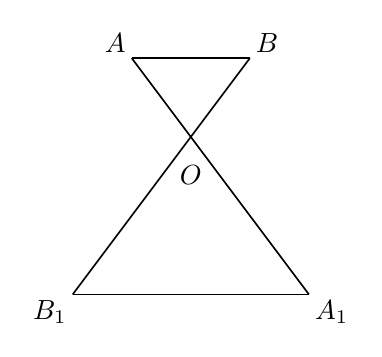
\begin{tikzpicture}[x=1cm,y=1cm,font=\normalsize,
 geometry edge/.style={solid,line width=.6pt},
 geometry mark/.style={solid,line width=.6pt},
 geometry label/.style={font=\normalsize,inner sep=2pt}]
\coordinate (A) at (-0.75,1);
\coordinate (B) at (0.75,1);
\coordinate (O) at (0,0);
\coordinate (B1) at (-1.5,-2);
\coordinate (A1) at (1.5,-2);
\draw[geometry edge] (A)--(B);
\draw[geometry edge] (B1)--(A1);
\draw[geometry edge] (A)--(O)--(A1);
\draw[geometry edge] (B)--(O)--(B1);
\node[geometry label,above left] at (A) {$A$};
\node[geometry label,above right] at (B) {$B$};
\node[geometry label,below,yshift=-8pt] at (O) {$O$};
\node[geometry label,below left] at (B1) {$B_{1}$};
\node[geometry label,below right] at (A1) {$A_{1}$};
\end{tikzpicture}
